\documentclass[a4paper,12pt]{report}
\usepackage{titlesec}
\usepackage{graphicx}
\usepackage{fancyhdr}
\usepackage{geometry}
\usepackage{indentfirst}
\usepackage{plantuml}
\usepackage{tikz}
\usepackage{aeguill}
\usepackage{float}
\usepackage{url}
\usepackage{hyperref}

% chktex-file 44

\newgeometry{
    top=2.5cm,
    bottom=3cm,
    inner=2cm,
    outer=2cm,
}

\pagestyle{fancy}
\fancypagestyle{plain}{}

\lhead{\scriptsize Computing and Information Technology\\
    2022\\
    David Daniel, Pava\\
    Walman: A Virtual Wallet Management System}
\rhead{
\includegraphics[width=4cm]{images/logo_upt.jpg}}
\cfoot{- \thepage\ -}
\renewcommand{\headrulewidth}{0pt}

\setlength{\headheight}{44pt}

\fancypagestyle{titlepage}{
    \lhead{\footnotesize Computing and Information Technology\\\textbf{2022}}
    \rhead{
\includegraphics[width=4cm]{images/logo_upt.jpg}}
    \cfoot{}
}

\titleformat{\chapter}{\center\normalfont\LARGE\bfseries\MakeUppercase}{\thechapter}{0.5em}{}
\titlespacing*{\chapter}{0pt}{3.5ex plus 1ex minus .2ex}{2.3ex plus .2ex}
\title{\LARGE WALMAN\\{ A Virtual Wallet Management System}}

\titleformat{\section}{\normalfont\large\bfseries\MakeUppercase}{\thesection}{0.5em}{}
\titlespacing*{\chapter}{0pt}{3.5ex plus 1ex minus .2ex}{2.3ex plus .2ex}
\title{\LARGE WALMAN\\{ A Virtual Wallet Management System}}

\author{Candidate: David Daniel, Pava
    \\Coordinator: Assoc. Prof.\ Razvan, Bogdan}

\date{June 2022 Session}

\begin{document}

\begin{titlepage}
    \thispagestyle{titlepage}
    \begin{center}
        \vspace*{10cm}
        \LARGE\textbf{Walman\\A Virtual Wallet Management System}\\
        \vfill
    \end{center}
    \begin{flushleft}
        \large\textbf{Candidate: David Daniel, Pava
            \\Coordinator: Assoc. Prof.\ Razvan, Bogdan}
    \end{flushleft}

\end{titlepage}

\chapter*{Abstract}

\tableofcontents

\chapter{Introduction}
In this project I implemented a wallet manager in the form of a mobile
application. The main features are password management, password generation, qr
and barcode storage and management, crypto wallet and OTP token management. The
user has the option to backup the data either in the cloud or on the
blockchain. Once backed up, the data will be available to be restored.

\section{Context}

\par In the last 30 years, the number of tasks that are digitalized has increased
exponentially. The most important part of the security systems of these tasks
is user management and authentication. The password is the most widely spread
form of user authentication and thus is often the prime target of attackers
that want to impersonate someone else.

According to~\cite{systematicAnalysis}, a \textit{``systematic literature
    review in the area of passwords and passwords security''}, there are many
problems with password security and management ranging from weak passwords and
password reuse, to users writing down passwords or sending them through
unsecure channels. Most of these problems according
to~\cite{systematicAnalysis} are solved by using password recommendations. A
good solution to most of these problems is a password management tool. A
password manager is a piece of software designed for generating and managing
passwords, in this way the user can have unique, complex and safely stored
password without having to remember them.

Another great method to better secure you accounts is using a two factor
authentication (2FA) method. These method vary from security questions, to one
time passwords (OTP) sent from the server to the user via email or SMS, to OTPs
generated using specialized algorithms such as: HMAC-based One Time Password
(HOTP)\cite{hotp} and Time Based One Time Password (TOTP)\cite{totp}.

The cryptocurrency market is another area that has seen a considerable
development lately. As of May 2022, the market cap of Bitcoin is around 565
billion USD, and the market cap of Ethereum is around 214 billion USD.\@ In the
case of Bitcoin, that is more than double of what it was in 2019 (around 211
billion USD), referenced in~\cite{cryptocurrencyMarketAnalysis}.
Cryptocurrencies also offer secure and long term storage capabilities thanks to
the blockchain technology. Blockchain backups, thanks to the decentralized
nature of the blockchain, are very hard to be tempered with. A traditional
cloud backup could be lost or inaccessible in more than one situations. The
most obvious one is data loss happening as result of a cyber attack or the
company simply going bankrupt. There are also situations in which the company
itself can refuse to serve you anymore. They can freeze your account or just
refuse to serve an entire country all-together, we have the recent example of
companies like Visa and Mastercard refusing to serve russian citizens as result
of political tensions as described in~\cite{russiaSanctions}
and~\cite{russiaSanctions2}. All these scenarios cannot happen in a
decentralized blockchain system.

Businesses that were traditionally not online like shopping also have inversely
digitalized. Nowadays most of the hypermarkets offer fidelity cards. Usually
these cards are built around a unique barcode or qr code. Often it's hard to
manage all your cards, so a digital storage solution to solve this issue would
help the end user better manage their cards.

Considered all mentioned above, a user has to remember and manage a lot of
information in order to interact with the currently available online
infrastructure. A tool that could help them manage all this data better is a
wallet manager.

\section{Motivation}

My personal motivation for creating a wallet manager is the fact that I want to
use it myself. Also I wanted for a long time to explore the state of the art in
smart contract development, so this was a great occasion to do so.

I chose to create this project in the form of a mobile application since people
tend to have their smartphones with them most of the time, so having a virtual
wallet on your mobile device makes sense.

Another factor that motivates me is the fact that currently in the mobile
application market there are almost no free and open source password management
applications available. The user needs to \textit{trust} the creators of the
application with their data, not knowing how the implementation of the product
is made, they have no guarantee that the data is safe.

\section{Similar Products Available on the Market}

There are a lot of password managers available on the market. In this section
we are going to try to make a comparison between some of the most popular
options available.

\begin{table}[h!]
    \centering
    \begin{tabular}{ | l | l | l | l | l | l | }
        \hline
        \textbf{Property}           & \textbf{LastPass} & \textbf{RememBear} & \textbf{KeePass} & \textbf{PassMan} & \textbf{KeyBase} \\
        \hline
        \textbf{Mobile Version}     & Yes               & Yes                & No               & Yes              & Yes              \\
        \hline
        \textbf{Blockchain Storage} & No                & No                 & No               & No               & Yes              \\
        \hline
        \textbf{Price}              & \$3/month         & \$6/month          & Free             & Free             & Free             \\
        \hline
        \textbf{License}            & Proprietary       & Proprietary        & GPL-2.0          & AGPL-3.0         & BSD-3            \\
        \hline
    \end{tabular}
    \caption{A comparison between some of the most popular password managers.}\label{tab:otherProducts}
\end{table}

In \autoref{tab:otherProducts} we have a comparison between some of the most
popular password managers available on the market. First off we have
LastPass\cite{lastpass} and RememBear\cite{remembear}, two very similar
password managers, both having a free and a payed plan. Neither of these two is
open source, so the most pressing issue regarding them is the guarantee that
your data is safe. Without having the ability to see how your data is managed
and stored you cannot be certain that it is secure. Also these applications do
not have blockchain backups.

KeePass\cite{keepass} is probably the most popular password manager for
desktop. It is free and open source, and the code was analyzed and certified by
specialized organizations such as the Open Source Initiative. The biggest
drawback to KeePass is the aged user interface and the missing mobile
application counterpart. Nowadays a lot of the situations where a user needs
access to their credentials are happening while using smartphones. Also the
features are limited, KeePass doing one thing and doing it well that being
password management. There are no cloud or blockchain backups, so the user
needs to manager backing up and storing their password database themselves.

Similar with KeePass, PassMan\cite{passman} is a free and open source password
manager. They have a mobile version of the application, but blockchain backups
are missing. Also, again, PassMan is just a password manager. It does not
manage shopping cards or crypto wallets.

Last but not least there is KeyBase\cite{keybase} which is not technically a
password manager. KeyBase is a blockchain, decentralized, social media
application. You can store password and secure notes inside the application but
from the user experience point of view, KeyBase was never designed to be a
password or wallet manager. The reason why it is mentioned, is because KeyBase
is implemented on the blockchain, all user data is encrypted and it's free and
open source.

\chapter{Technology Stack}

In this chapter I am going to describe the technologies used. The application
has 3 main components. The first component is the frontend, a mobile
application. The second one is the cloud storage backend. The last part are the
smart contracts deployed on the blockchain.

\section{Frontend}

The most important aspects I considered when I chose the technologies used for
the frontend was cross-platform capabilities, ease of testing, documentation
availability and performance. This is why for this project I chose a Flutter
stack.

\subsection{Flutter}

Flutter\cite{flutterDocs} is a mobile application development framework
developed by Google in the Dart programming language. It was released in May
2017 and it currently is one of the most popular mobile development frameworks.

According to \textit{``An empirical investigation of performance overhead in
    cross-platform mobile development frameworks''}\cite{flutterPerformance},
Flutter has one of the better resource management systems when compared with
other popular mobile development frameworks.

\begin{figure}[H]
    \centering
    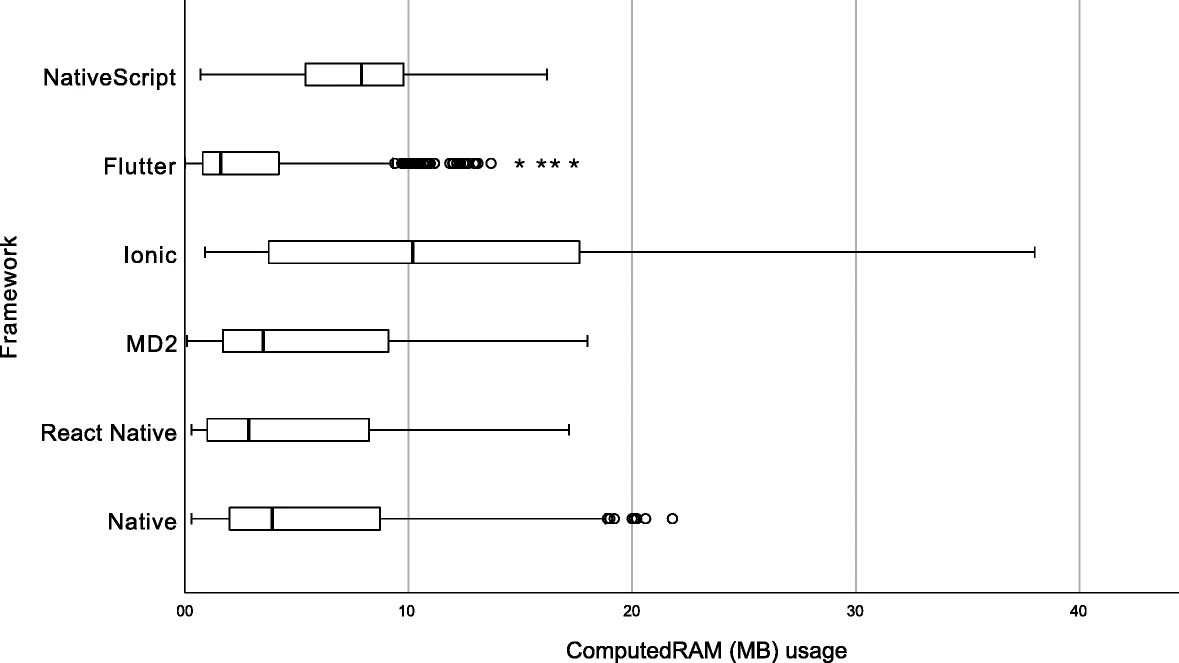
\includegraphics[scale=0.4]{images/flutterPerformance/ram.png}
    \caption{Boxplot from~\cite{flutterPerformance} of RAM usage across all tests done in~\cite{flutterPerformance} }\label{fig:flutterPerformanceRAM}
\end{figure}

As seen in~\autoref{fig:flutterPerformanceRAM}, on average Flutter outperforms
most of the other frameworks in memory management.

\begin{figure}[H]
    \centering
    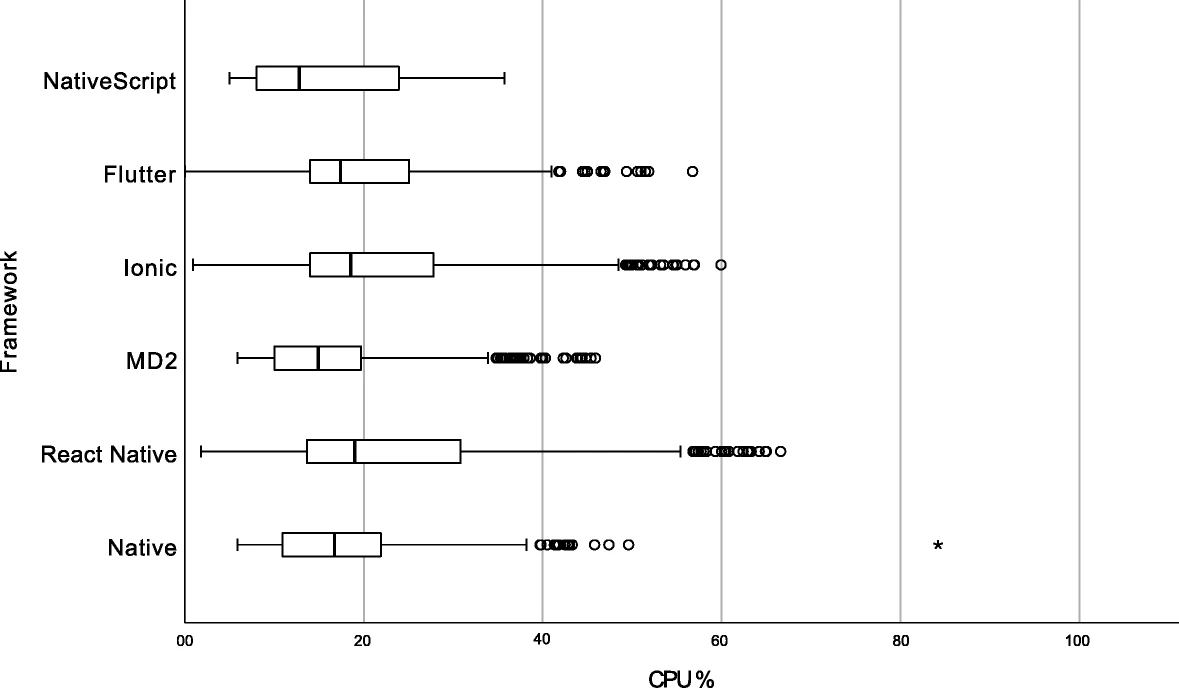
\includegraphics[scale=0.4]{images/flutterPerformance/cpu.png}
    \caption{Boxplot from~\cite{flutterPerformance} of CPU usage across all tests done in~\cite{flutterPerformance} }\label{fig:flutterPerformanceCPU}
\end{figure}

In~\autoref{fig:flutterPerformanceCPU} we have a comparison between CPU usage
of similar applications implemented in different frameworks
in~\cite{flutterPerformance}, where Flutter achieves a competitive result when
compared to the other frameworks.

Another very important feature of Flutter is cross-platform compatibility. A
mobile application developed in this framework can be build in native Android
and IOS applications with minimal performance loss. There is also Flutter Web
for web applications, offering the option to create a browser variant of the
application in the future, reusing already developed and tested parts from the
mobile application.

Flutter comes with a very rich and detailed documentations, the Flutter
Docs\cite{flutterDocs} and a set of development plugins for the most used IDE
and text editors such as Android Studio, Intellij or Visual Studio Code. During
the development process the code is executed into a runtime environment,
allowing almost instant compilation times speeding up the development, and in
production, the code is compiled into a native application for performance
enhancement.

The User Interface in Flutter is build based on a widget tree, similar to
React. Every User Interface item inherits the Widget class.

\subsection{Dart}\label{chapter:dart}

Dart\cite{dartDocs} is a general purpose programming language developed by
Google starting with 2011. It was intended to replace JavaScript and TypeScript
for frontend applications, but instead, later, it was used to create the
Flutter framework.

Dart is a type safe, C-like programming language. It can be both interpreted by
a runtime or compiled. The memory management is handled by a garbage collector
similar with Python or JavaScript.

One of the strongest features of Dart is the compiler. It can be compiled in
binary code, JavaScript or mobile native code such as Java and Kotlin for
Android and Objective-C and Swift for IOS devices. Dart also performs tree
shaking at compile time, discarding unused objects, methods and functions.

\subsection{Code Generation}

During the development of the project I used multiple packages (dart libraries)
in the process. One very important package that needs to be mentioned is the
\textit{freezed} package\cite{freezedDocs}. This offers code generation for
common model functionalities such as json encoders and decoders, copyWith
methods, different constructors and access functions and more.

Classes generated by the package are annotated with the \textit{@freezed} tag.
The generated code is stored into files that contain the \textit{.freezed.dart}
and \textit{.g.dart} extensions.

\subsection{State Management}

One of the most important aspects of frontend application development is state
management architecture. There are a lot of different state management patterns
available in Flutter\cite{flutterStateManagement} such as Provider, BLoC or the
simple setState. These state management patterns tell the application when the
state has changed and when certain components of the presentation layer (the UI
of the application) needs to be updated as a result of that.

For this project I used the Redux state management architecture. This pattern
is a very popular solution for managing the state of an application, and it is
commonly used in web development. There is an implementation for it in Flutter
in the packages: flutter\_redux\cite{flutterReduxDocs}, redux\cite{reduxDocs}
and redux\_epics\cite{reduxEpicsDocs}.

\begin{figure}[H]
    \centering
    \scalebox{0.75}{\input{diagrams/component/redux.latex}}
    \caption{Basic structure of a Redux State Management System}\label{fig:reduxArchitecture}
\end{figure}

In~\autoref{fig:reduxArchitecture} we can see the core structure of the redux
architecture I used in the project. A state change begins the dispatch of an
action. They are usually triggered by the user interface, but in some cases
they can be triggered by an API event. The Epics are a set of listeners which
analyze the action stream. When an Epic recognizes an Action, it performs a
series of operations which can process the data using the APIs (business logic)
or dispatch new actions. Every action is also watched by the Reducer, which
listens for Actions and changes the State accordingly. When the State changes,
the Widgets (in case of Flutter) that depend on the elements updated in the
State, are triggered to pe updated.

In order to access specific elements of the state, and not update every widget,
every time the state changes. Containers can be used to access a specific part
of the state. In order to access the State, the User Interface needs to request
it from the Store, in this way, the Store knows when to redraw the object. The
widgets that update when the state is modified and have access to the Store are
part of the flutter\_redux package\cite{flutterReduxDocs}.

Error handling in redux is made using special stream functions from the RxDart
package\cite{rxDartDocs}. RxDart offers and extension to the functional
capabilities of dart. In redux the application is represented as a stream of
actions. In order to make error handling efficiently, every action sequence
spawns a new stream. In case of an exception, the stream will have an exception
and we can dispatch a new Action with relevant information about the error. In
this way the probability of total application wide runtime exceptions is
dramatically lowered.

\section{Firebase}

In this section I am going to describe the technologies used for the creation
of the cloud storage server portion of the application. In order to use the
cloud storage, the user needs to create an account. After the account is
created, the user needs to have the ability to create backup entries and
restore previous backups.

Firebase\cite{firebaseDocs} is an app development platform created by Google,
designed as a backend for mobile and web applications. Firebase offers already
implemented solutions for user management, artificial intelligence integration
and databases. A firebase backend is hosted by Google in a ``pay as you use''
monetization scheme.

For this project I chose to use the services provided by Firebase to implement
the cloud storage part of the project, mainly for ease of deployment, the good
integration with Flutter throughout the dedicated packages and reduced costs
(so far free).

The user management uses the email and password login service provided by
Firebase. Once a user account is created, a database entry is also made, access
to this database being restricted to the user base on their unique identifier.

For the storage, Firebase provides two different services. The first one is
Real Time Database, which is a NoSQL type database, that resembles a Json type
file. There are drawbacks to the Real Time Database such as low fragmentation
which increases the data transfer size between the client and the server. A
solution to this problem is the second service, Firestore, which is also a
NoSQL type database similar with Real Time Database but it has some additional
features. Firestore is structured into collections of documents which each have
multiple fields of different types. This approach allows the client a more
granular access to the data, reducing the size of files transferred between the
client and the server and client side processing.

\section{Blockchain}

For the Blockchain storage of the application I used the Ethereum smart
contract development stack with Solidity. In this chapter I am going to explain
the basic logic behind the blockchains, how smart contracts are built into them
and the economy between smart contract deployment and usage.

\subsection{What is a Blockchain?}

The blockchain is the basic structure that sits at the base of most of the
cryptocurrencies. At it's core, it is a decentralized, distributed system of
data storage and processing.

\begin{figure}[H]
    \centering
    \scalebox{1}{\input{diagrams/deployment/block.latex}}
    \caption{The structure of a block as described by the Ethereum documentation\cite{ethereumDocs}}\label{fig:block}
\end{figure}

The blockchain is made up of a list of blocks connected to each other. Every
block contains a set of information about itself and a reference to the
previous block, the \textit{parentHash} field in case of Ethereum, in the form
of a hash as described in~\autoref{fig:block}. The \textit{parentHash} of the
current block is the \textit{mixHash} of the previous block.

The \textit{mixHash} is the digest of a hashing algorithm of the entire content
of the block. The \textit{mixHash} needs to have the first two bytes 0, in
order to be considered mined. This is achieved by incrementing the
\textit{nonce} field until the target \textit{mixHash} is reached.

For the hashing algorithm, Ethereum was developed using the Keccak-256 hashing
function, which was later standardized as SHA-3 in~\cite{sha3}.

The block also has the \textit{timestamp} when it was mined and the
\textit{stateRoot} which contains metadata about the current state of the
system.

Information about the difficulty of the mining process and the respective price
of the process are also stored in the block, in the \textit{difficulty} and
\textit{baseFeePerGas} fields.

The \textit{transactions} field contains information about the transactions
associated with the block and the optional data exchanged. This is the place
where the smart contract logic is deployed and later interacted with.

A successfully mined block is added to the blockchain and then the transaction
is confirmed by every subsequent blocks.

\begin{figure}[H]
    \centering
    \scalebox{1.1}{\footnotesize\input{diagrams/object/blockchain.latex}}
    \caption{High level relationship between two blocks}\label{fig:blockchain}
\end{figure}

In~\autoref{fig:blockchain} the relationship between two blocks is represented.
As stated before, \textit{block 2} has the mixHash of \textit{block 1} in it's
parentHash field. In this example, \textit{block 1} being the first block in
the blockchain has the null value as parentHash.

If the data in \textit{block 1} was to be changed, it would invalidate the
mixHash of \textit{block 1}. The mixHash would have to be mined again, but then
it will be different thant the parentHash of \textit{block 2}, therefore
invalidating the blockchain. This is the first mechanism of defense against
malicious data manipulation. There cannot be changes in any previous blocks of
the blockchain without invalidating every block starting from the change.

The blocks following a changed block can be mined again in order to re-validate
the blockchain. Here is where the second line of defense comes in,
distribution. Every chain is stored on multiple nodes, therefore a change in
one has to be reflected in all of them. This makes data alteration nearly
impossible.

\subsection{Ethereum}

Ethereum is one of the most popular cryptocurrencies. Other than the popularity
and the implicit high amount of resources that is implied, and unlike other
popular cryptocurrencies like Bitcoin, Ethereum offers the ability to run code
on the blockchain using the Ethereum Virtual Machine (EVM)\cite{ethereumDocs}.

Every execution on the Ethereum Virtual Machine requires Gas, which is an
amount of Ethereum cryptocurrency units (ETH) proportional with the complexity
and the memory requirements of the task. Since the cost of an ETH has raised
dramatically over the last 5 years, subdivisions of the currently were created.
The two most widely used subdivisions are \textit{wei} (\(10^{-18}\) ETH) and
\textit{gwei} (\(10^{-9}\) ETH).

Since the development of a blockchain application implies a lot of testing and
prototyping, solutions of simulating the blockchain were created. Ganache is
such a software developed in JavaScript, it simulates an Ethereum blockchain on
a local machine or on a server. For this project I tinkered with Ganache but
later I decided to go one step further and deploy my contracts on an Ethereum
Testnet.

Ethereum Testnets are networks similar with the main Ethereum network
(mainnet), designed to provide a free of charge development environment
identical with the mainnet. Testnets are blockchains that run in parallel with
the mainnet, having the same functionalities and features. There are a lot of
Ethereum Testnets like: Ropsten, Kovan or Goerli. In this project I worked with
the Rinkeby network. Unlike on the mainnet, ETH is generated constantly on the
Testnets and it is distributed to any wallet that requests it via faucets.
There are no costs involved with developing a blockchain application on a
Testnet. After the development process is complete, in production the
application can be easily redeployed on the mainnet.

\subsection{Smart Contracts}

The code that can be executed by the Ethereum Virtual Machine has to be
compiled into a specific binary code. Smart contracts are transactions that
contain binary code that can be later executed from subsequent transactions.
Gas cost afferent to the execution of the contract is payed by the transaction
that wants to execute the contract, not the contract itself. Therefore in order
to create a blockchain application, one of the requirements of such a program
is having an attached cryptocurrency wallet. In the case of server
applications, this wallet can be a server secret, managed by the administrator,
but in the case of client applications, the wallet cannot be incorporated by
default into the application, since that would mean that everyone has access to
it and is able to act maliciously. This is is the reason why this project
requires an integrated wallet. An external wallet can also be used, but it
would deteriorate the user experience.

Once a smart contract is deployed, it cannot be changed, therefore testing such
a contract for vulnerabilities and bugs is essential.

One very important aspect of blockchain applications is gas efficiency. Certain
operations consume more gas than others, and storing data also consumes gas.
The application should be optimized to leave a minimal data footprint focusing
on using non persistent memory.

Accessing data from a smart contract is free of charge. As long as there is no
new data to be stored or there is no code to be executed, accessing the data in
a smart contract is cost free.

A very important security aspect of smart contracts and blockchains in general
is that data is always visible by anyone who accesses the blockchain and it
cannot be modified. Therefore sensitive data needs to be encrypted.

\subsection{Solidity}

Solidity\cite{solidityDocs} is a dedicated programming language for blockchain
applications. It was designed specifically for the creation of smart contracts.
This language is an object oriented, compiled language that resembles C++ and
JavaScript.

Code written in Solidity is compiled into binary code that can be executed on
the Ethereum Virtual Machine and there are specific modifiers for the
interaction with the EVM and code optimization. Some of these modifiers are:
\textit{view} which specifies that the afferent function is forbidden from
changing the state and \textit{payable} which allows ETH to be transferred with
the function call. There are also more commonly used modifiers like:
\textit{override}, \textit{virtual}, \textit{private} or \textit{public}.

\section{Development Environment}

For the creation of this project I used a wide variety of tools. They range
from Integrated Development Environments (IDEs) to task management
applications.

For the development of the mobile application I used Intellij and Visual Studio
Code with the Flutter specific plugins. I also used Adobe XD for user interface
design and plantuml for diagrams. In order to test the application, I used the
Android Virtual Machine provided by Android Studio.

For the blockchain part of the application I wrote the smart contracts using
Solidity. I created a python compilation script for the smart contracts that is
also used in the testing pipeline.

For the cloud portion I used the Firebase console and the specific packages for
Flutter.

All the code was managed using the Git software versioning system and it was
deployed on Github at \url{https://github.com/dvpv/walman}. I used the Github
Actions feature in order to manage the two test pipelines for the mobile
application and blockchain smart contracts.

The smart contracts were deployed on the Rinkeby Testnet using the Remix
Ethereum IDE, and in order to access them from the mobile application, the
web3dart\cite{web3dartDocs} flutter package was used.

For task management I used Focalboard, a free and open source alternative to
Trello.

\chapter{Implementation}

\section{Use Cases}

The application has six main components: the password, qr and barcode, OTP and
crypto-wallet managers and the cloud and blockchain backup solutions.

\begin{figure}[H]
    \centering
    \scalebox{0.45}{\large\input{diagrams/usecase/usecase.latex}}
    \caption{Principal use cases of the application}\label{fig:useCase}
\end{figure}

In~\autoref{fig:useCase} the main use cases of the application are depicted.

The entire application is locked and encrypted using the mater key. If a master
key was not set yet, in the case of a first time launch of the application, the
user is prompted to create a new master key. After the application is unlocked,
the user has access to multiple functionalities and features.

The home page of the application shows in a short format the passwords, codes
and wallet balance. The user can navigate to different pages for each of the
functionalities.

The passwords page, shows the user a list with the passwords that are currently
stored into the database. Here the user has the option to add, edit or remove
passwords.

The codes page is similar with the passwords page, the user has the ability to
scan new codes, view existing ones and delete them.

On the OTP page, the user can see the currently stored one time passwords. The
codes are updated every second and a timer representing the remaining time in
which the current code is valid is displayed.

On the wallet page, the user can see the current balance of the wallet and the
public address. The only transactions that can be made with this wallet are
blockchain backup operations.

The sync page shows all available cloud and blockchain backups. The use has the
option to restore a backup, or create new ones.

In order to create a blockchain backup the user needs to have a crypto wallet.
If there is no crypto wallet created, the user has the option to import one by
private key or create a new one. For the backup to work, the wallet needs to
have enough currency in it in order to pay for the gas price. Restoring a
backup requires no gas payment. Crypto wallets are not backed up on blockchain
backups and neither they are on cloud backups.

For a cloud backup to be created the usr needs to be logged into a cloud
account. If the user is not yet logged in, they can create new account, or
login into an existing one.

On the settings page, the user can manage the cloud account and view and delete
the wallet private key.

There is an app-wide search button which displays results from the entire
application. If the user clicks on one of the results, they will be redirected
to the respective page in order to view the content.

\newpage
\section{System Architecture}

The system in composed out of three main components. The communication between
these components is made exclusively using the HTTPS protocol.

\begin{figure}[H]
    \centering
    \scalebox{0.499}{\large\input{diagrams/component/system.latex}}
    \caption{High level system architecture}\label{fig:system}
\end{figure}

In~\autoref{fig:system} a high level representation of the system is depicted
into a component diagram. The user can directly interact only with the mobile
application. The Firebase component is deployed online in the cloud platform
provided by google and the smart contract is deployed on the Ethereum
blockchain.

The mobile application is the first component and it is the only component that
initiates data exchange in the system. It has three API sub components for each
of the online services it needs to communicate with and one API for interaction
with the Secure Storage.

The Secure Storage (or Secure Enclave on IOS) is a special persistent memory
zone created to store sensitive information on a mobile device. I used the
Secure Storage to save the part of the application state that needs to be
recovered at each application start.

The middleware consists of the redux epics defined into the application. The
epics are the only part of the mobile application which has access to the
external APIs.

The user interface interacts with the middleware by dispatching redux actions.
The state of the application is updated by the reducer when it detects specific
action events that require a state update. The user interface code is
completely separated from the APIs, the only connection being the middleware.

\section{Application Flow}

\begin{figure}[H]
    \centering
    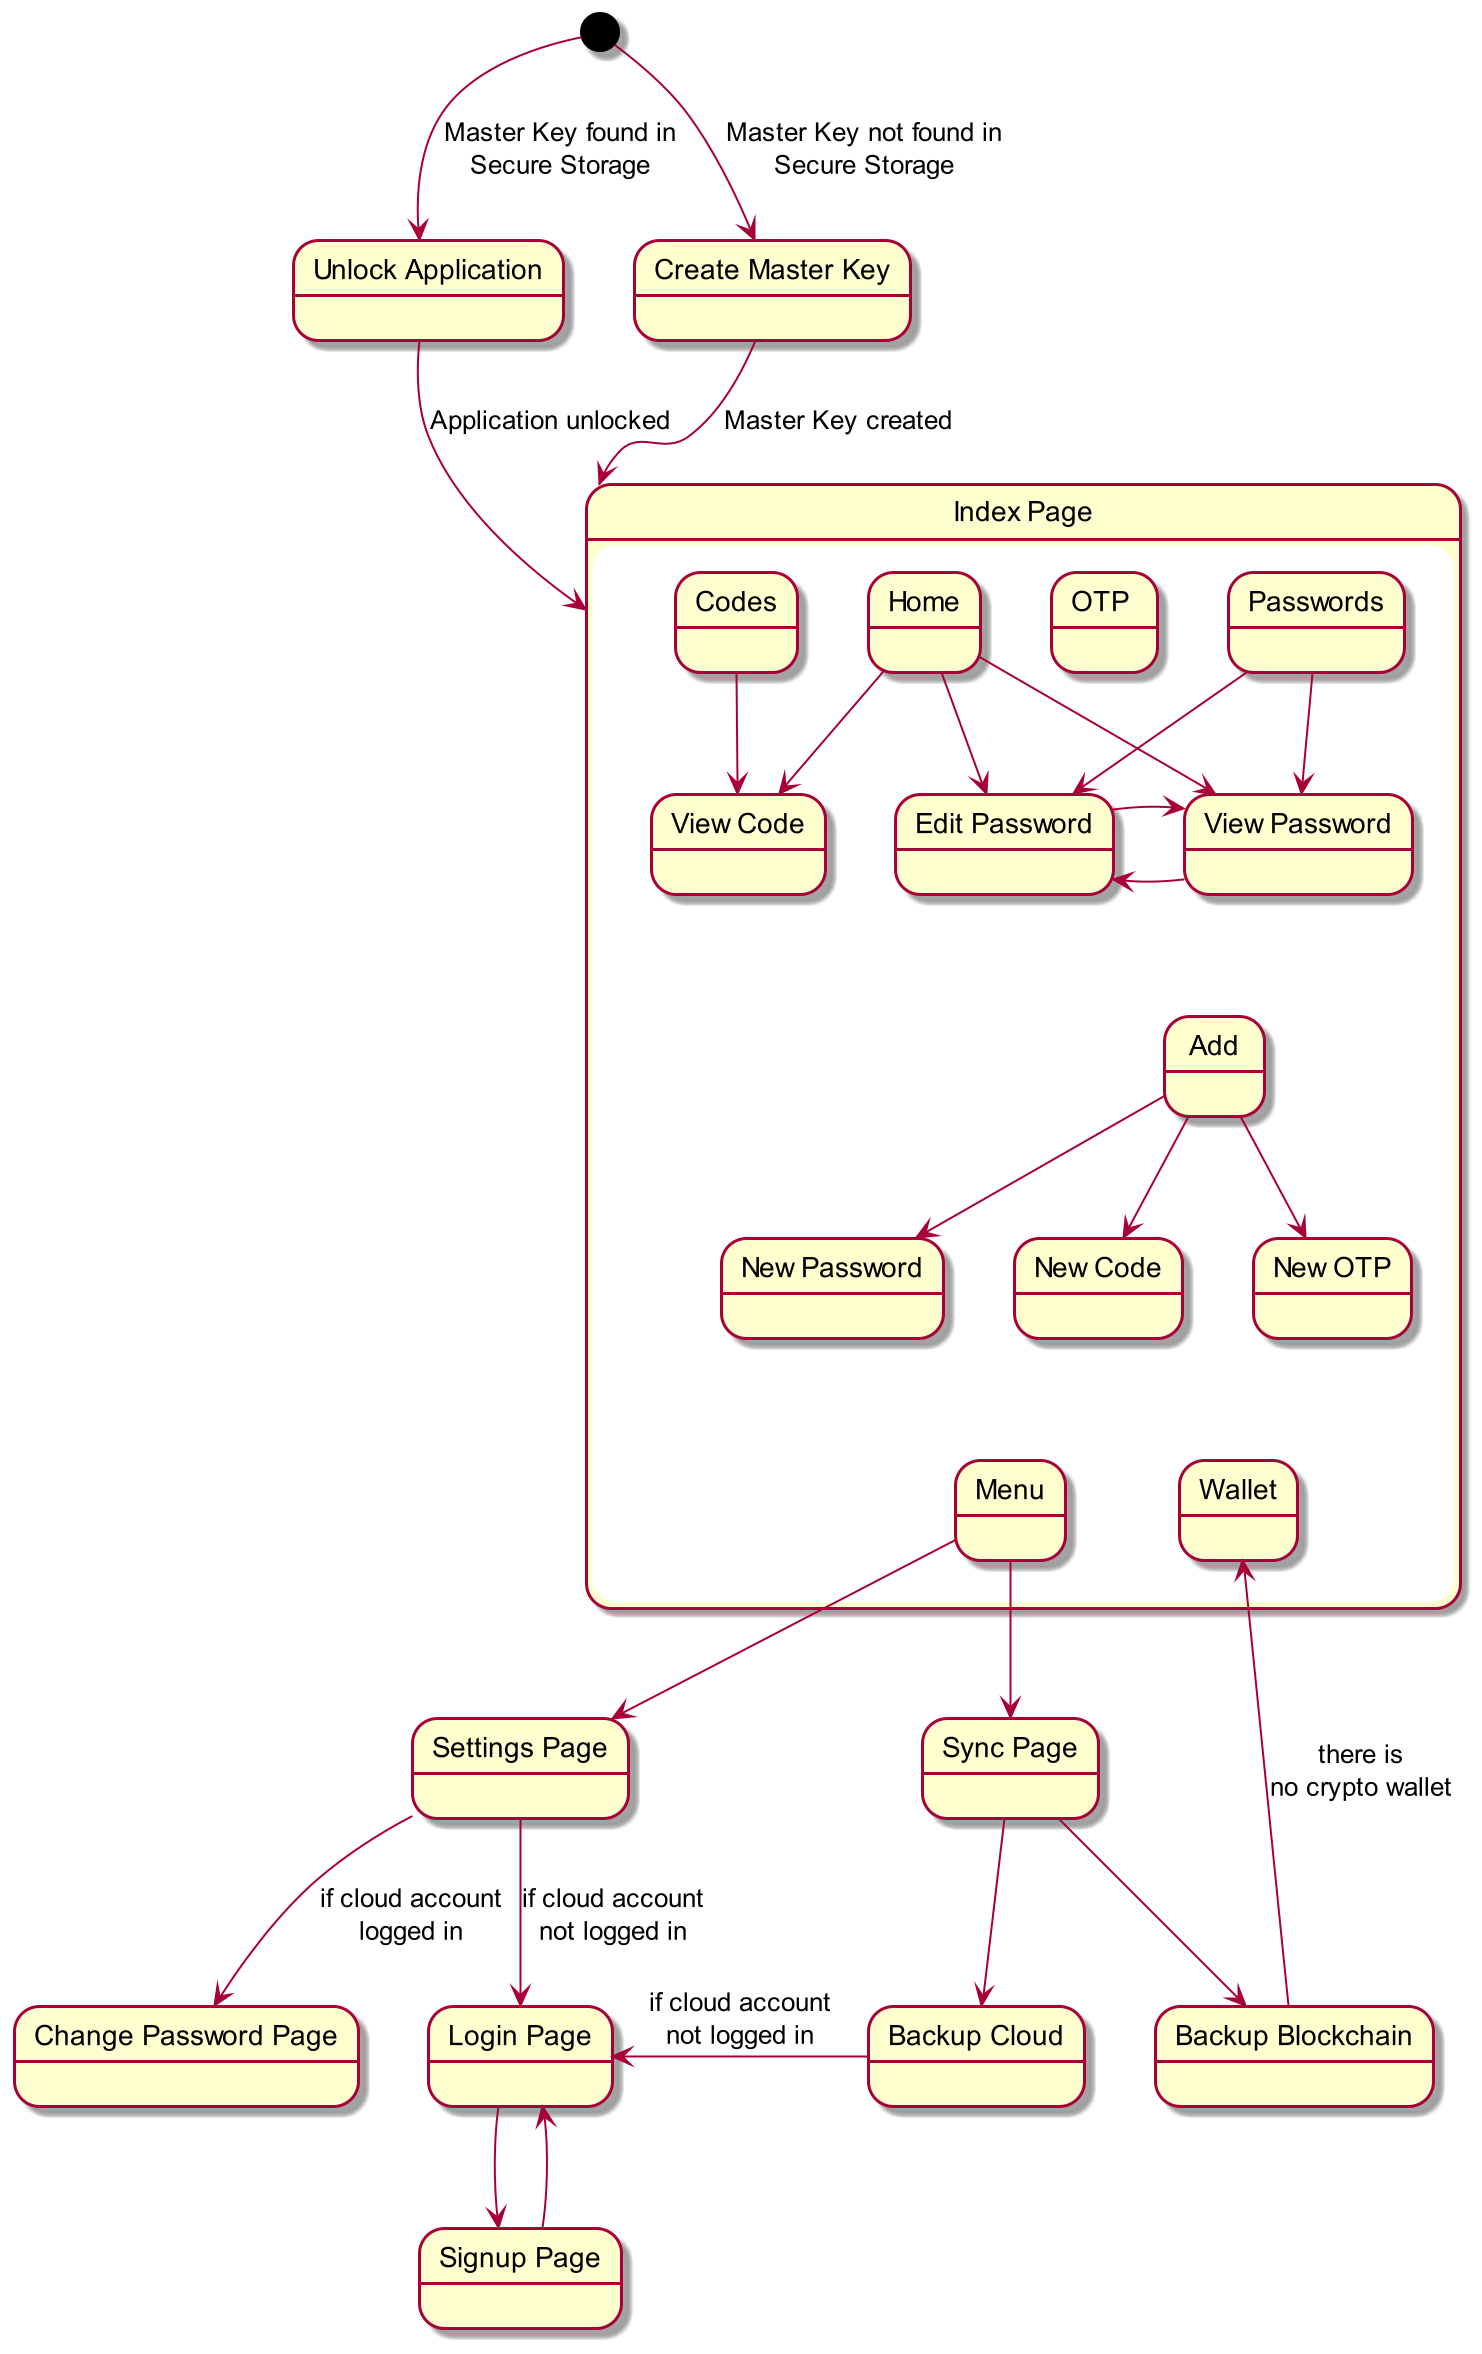
\includegraphics[scale=0.23]{diagrams/state/flow.png}
    \caption{Flow diagram showing the main pages and fragments of the application}\label{fig:flow}
\end{figure}

In~\autoref{fig:flow} we can see the flow between the main elements of the user
interface. Initially the user needs to input the master key in order to unlock
the application or create one if it does not exist.

\begin{figure}[H]
    \centering
    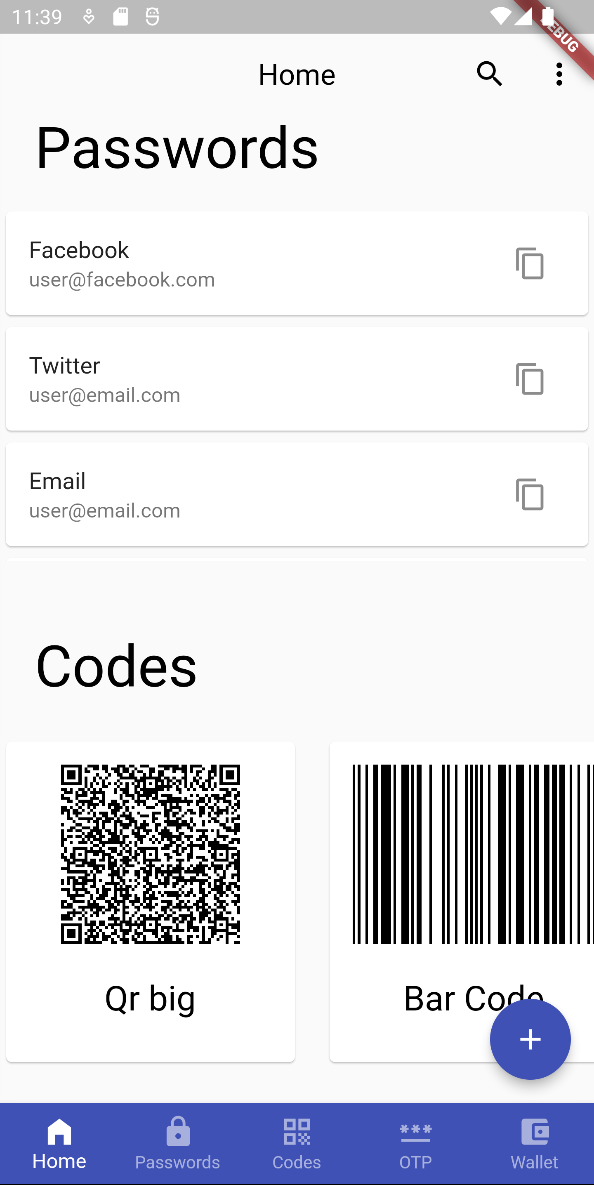
\includegraphics[scale=0.4]{images/app/home.png}
    \caption{Home fragment of the application}\label{fig:homepage}
\end{figure}

After the application is unlocked the user is redirected to the Home
fragment,~\autoref{fig:homepage}, of the Index page. Here the user has quick
access to passwords, codes and the wallet balance. The user can navigate
different fragments using the bottom navigation bar. The passwords fragment
contains a list with all the passwords. Here the user can copy the passwords if
they tap on the copy button of a password. On long tap a context menu giving
the user the delete, edit and copy options shows up. On tap a password opens a
details page containing information about the password. From this page the user
can go to the edit page where they can change the data related to the selected
password.

The Codes fragment is similar with the password page. It shows a list that
contains all the codes. If the user taps on a code, a details page will be
opened showing a big picture of the code and it's content. The user can delete
the code in the details page or in the Codes fragment by log tapping and
selecting the delete option in the context menu.

The OTP fragment shows a list containing all the stored tokens and the current
code for each. If the user taps on one of these list entries the code will be
copied to the clipboard. The user can delete an OTP token by selecting the
delete option from the context menu after a long tap on a token.

The last fragment is the Wallet. Where if there is no wallet created yet, the
user can create a new wallet or import one by introducing the private key. When
a wallet exists the balance of the wallet and the public address are displayed.

On the top right of the Index Page there is a menu, seen
in~\autoref{fig:homepage}. This menu offers the user the option to open the
sync page, the settings page or the password generator.

\begin{figure}[H]
    \centering
    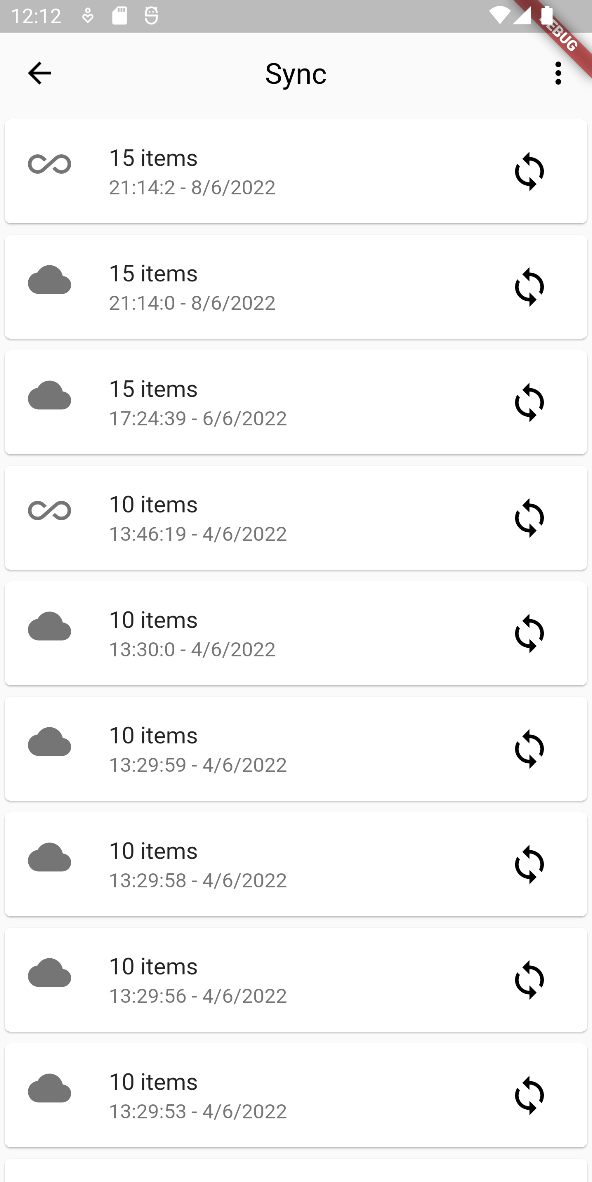
\includegraphics[scale=0.4]{images/app/sync.png}
    \caption{Sync page of the application}\label{fig:syncpage}
\end{figure}

The sync page,~\autoref{fig:syncpage}, contains a list with all the available
backups the user can restore. A backup can be restored by pressing the restore
button of the desired backup. Every backup has the number of items displayed
and also the date and time when it was created is also shown. The backups are
sorted chronologically, the most recent ones being at the top. The blockchain
backups are represented by an infinity icon and the cloud ones by ca cloud
icon.

In case there are no backups available the user is prompted with the option to
create one instead of being shown an empty list. The user can also create a
backup by selecting the appropriate option form the top right menu.

If the user tries to create a blockchain backup but there is no wallet set,
they are redirected to the wallet fragment of the index page. Where they are
prompted to create or import a wallet.

Similar, in the case when the user wants to create a cloud backup but they are
not logged into a cloud account, they are redirected to the login page and
prompted to login or signup for the cloud service. After the login process is
done they are redirected back to the sync page and a cloud backup can now be
created.

\begin{figure}[H]
    \centering
    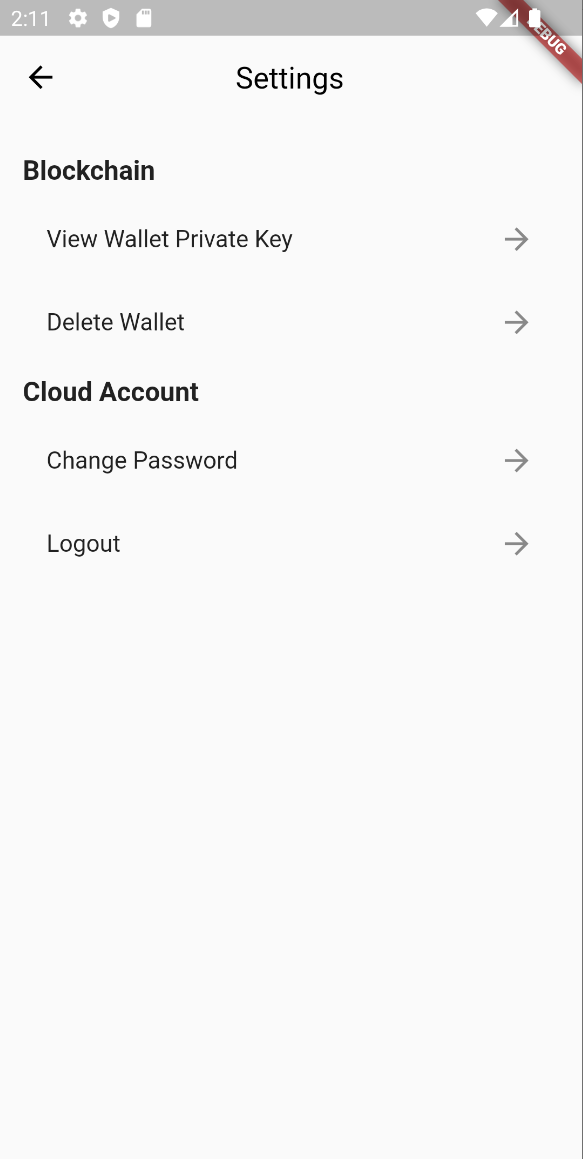
\includegraphics[scale=0.4]{images/app/settings.png}
    \caption{Settings page of the application}\label{fig:settings}
\end{figure}

The settings page,~\autoref{fig:settings}, can be accessed form the index page
menu. Here the user can delete or view the wallet private key and manage their
cloud account. The settings page changes depending on the state of the
application. If the user did not create or link a wallet yet, the settings page
will display the options to do so instead of the delete and view ones. If the
user did not login to the cloud account yet the settings page will display a
login option.

\section{Application State}

The application state is responsible for storing the data the application works
with. This data is needed to build the user interface.

As stated in the \textit{Technology Stack} chapter, the state management system
used in this application is Redux. Unlike in other architectures like BloC, in
this pattern the entire application has only one state object that contains all
the information.

Each time the state is updated, the user interface is rebuilt as well. In order
to selectively rebuild the user interface components, containers are used.
Containers are specific providers that select only one object from the AppState
class that is used to build the user interface. If there are more than a single
element from the AppState needed to build a part of the user interface, nested
containers can be used. Each time the container detects that the represented
data has changed, it rebuilds the afferent user interface. Implementation for
containers is partly provided by the flutter\_redux
package\cite{flutterReduxDocs}.

\begin{figure}[H]
    \centering
    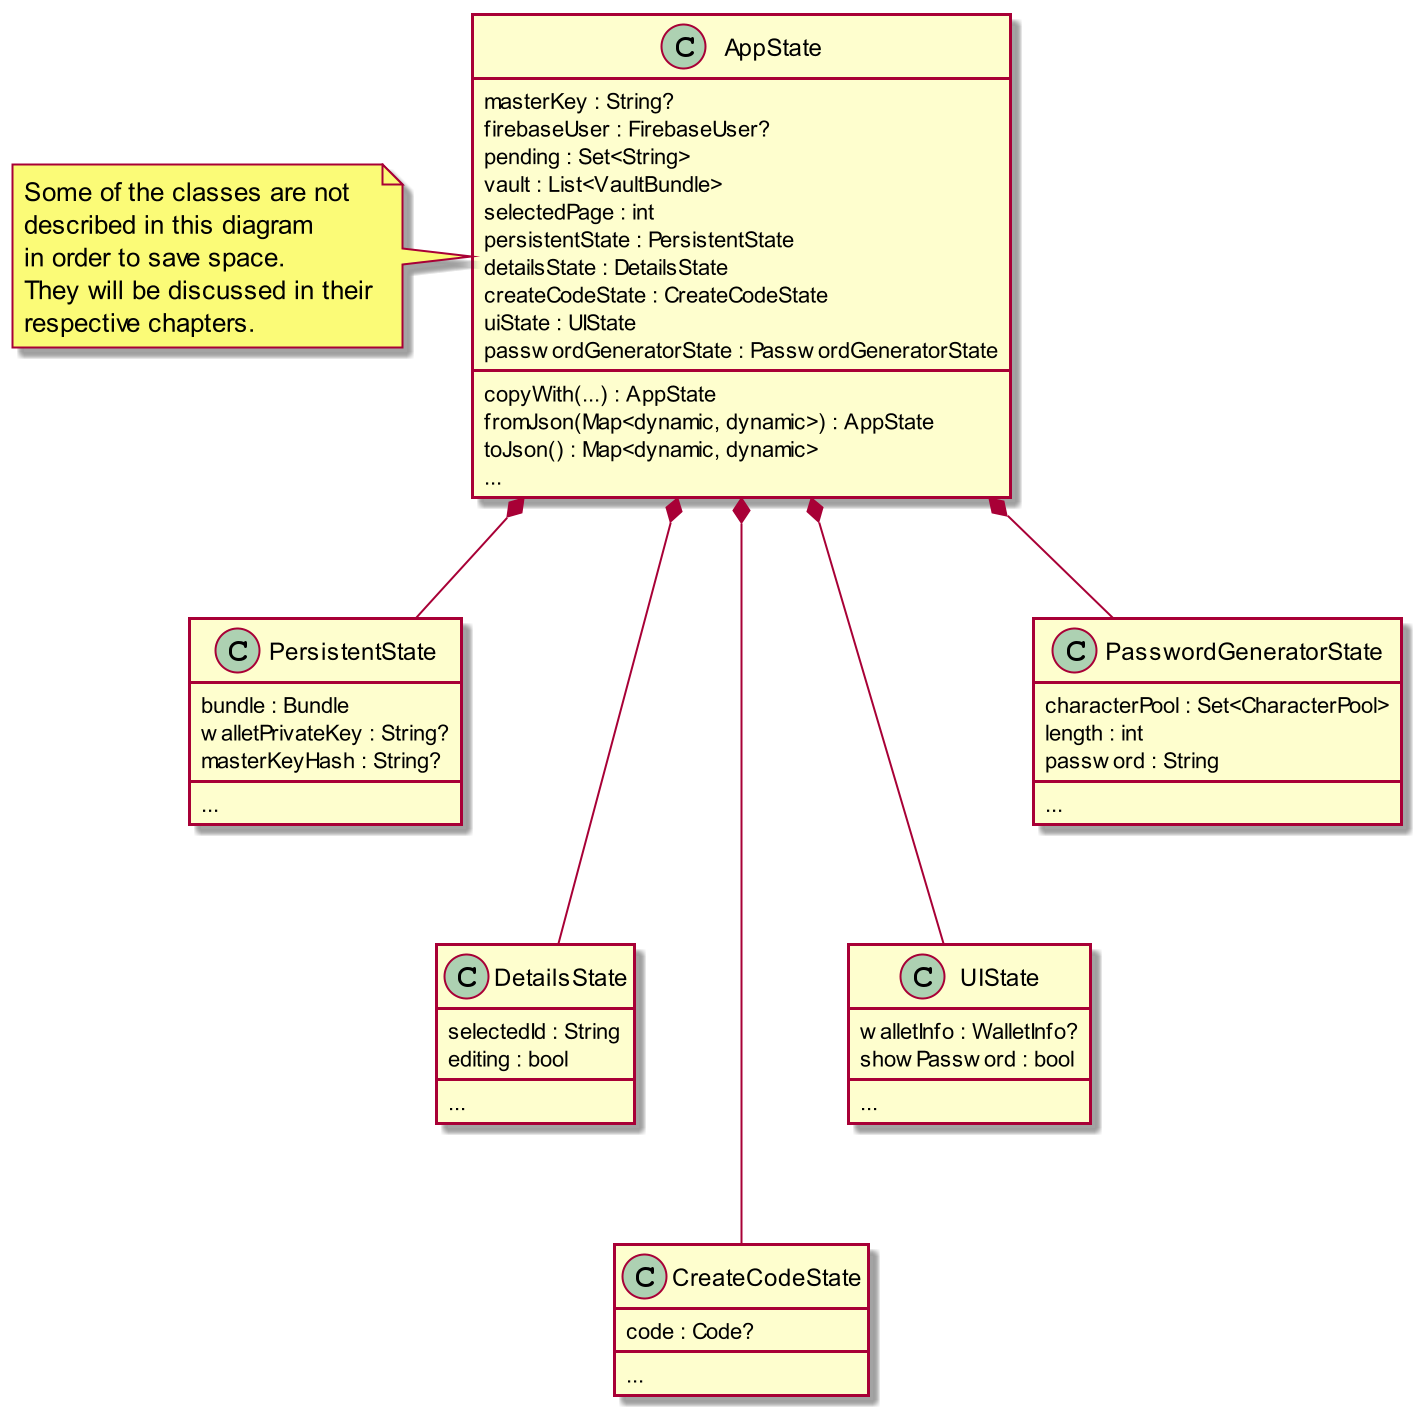
\includegraphics[scale=0.33]{diagrams/class/app_state.png}
    \caption{Class diagram of the AppState model}\label{fig:appstate}
\end{figure}

The AppState model is described in~\autoref{fig:appstate}. This model is
composed of five other state classes. In Dart `\textit{?}' next to some
variables signifies that the specific type is nullable and the null value can
be assigned to it.

First we have the master key in the form of a nullable string. At the start of
the application, the master key is null and after it was verified with the
master key hash from the persistent state, it is set to the appropriate value.

The \textit{firebaseUser} field contains data about the cloud user account if
it exists. In case the user is not logged into the cloud account the field is
null.

The set of pending strings is used to signal to the user interface when some
special actions processes are ongoing. These actions have a specific pendingId
which is added to the set when they are dispatched and removed when the final
action is completed. This helps makes it so the user interface can show
progress indicators to the user when an operation is ongoing.

All the fetched backups form the cloud and the blockchain are stored inside the
state into the \textit{vault} list. The VaultBundle type contains a timestamp
at which the backup was made and a `Bundle' which is a an object containing the
passwords, OTP tokens and codes of the application at one point in time and it
will be described in more detail in another chapter.

The \textit{selectedPage} integer represents which fragment will be shown on
the index page.

The persistent state is the data of the state that needs to be stored using the
Secure Storage API into permanent memory so it will be loaded back when the
application is restarted. In this state we keep the `Bundle' with the current
database, the master key hash and the private wallet key. Everything except the
master key hash is encrypted with the master key itself and decrypted after the
user unlocks the application.

The details state is a small state used when the password details page is
displayed.

When the user scans a new QR, barcode or OTP token, the result of the scan
operation is temporally stored into the \textit{code} field of the
CreateCodeState.

The UIState is used to store information that is only relevant to the user
interface and it's not used when calling the APIs.

The last part is the password generator state which contains the options of the
generator and the generated password.

All the states are immutable and in order to be changed, a new state is
created. This is done using the \textit{copyWith} method which as arguments has
all the fields form the class as nullable types. If a field is nullable and it
is not preceded by the \textbf{required} modifier, it is an optional field with
the default value null. If the \textit{copyWith} function does not receive a
parameter, it defaults to the value that the object stores at the moment of the
call. The method returns an object of the same type as the class it is
contained in.

The \textit{copyWith} function as well as some more utility functions like json
encoders and more, are automatically generated using the
freezed\cite{freezedDocs} package. There are no issues with having methods that
are not used in the final code since Dart has the tree shaking feature which
automatically drops unused code components, and form the maintenance point of
view there are no issue since this is generated code, tested by the package
itself.

\section{Application Action}

\begin{figure}[H]
    \centering
    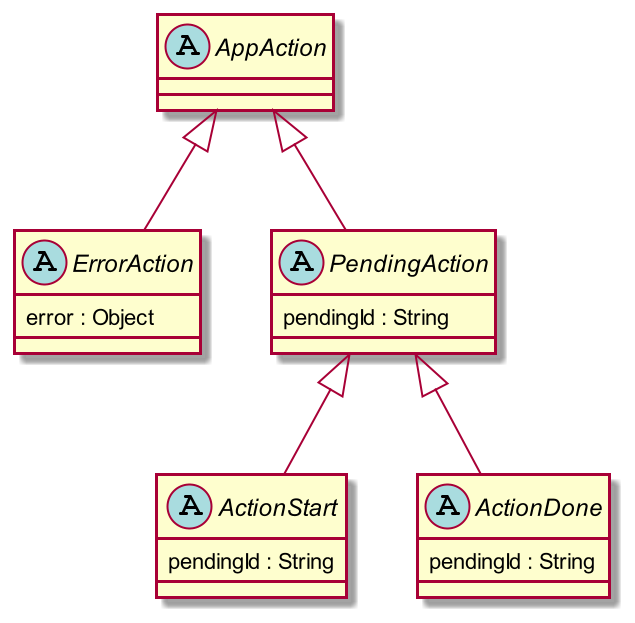
\includegraphics[scale=0.45]{diagrams/class/app_action.png}
    \caption{Class diagram of the AppAction model}\label{fig:appaction}
\end{figure}

The application action is the base type for the action events. These actions
are dispatched by the user interface as result of user interaction and they are
intercepted into the epics and reducers where they trigger API calls and state
change respectively.

In~\autoref{fig:appaction} we can see the inheritance relationship between the
action base types. The \textit{AppAction} class is the base of all actions and
it is detected by the reducers and epics.

The \textit{ErrorAction} class is used when an action failed due to an error.
When an action stream crashes, an \textit{ErrorAction} type object is emitted
by the epic.

The \textit{PendingAction} types \textit{ActionStart} and \textit{ActionDone}
contain a specific pendingId of the action that implements them which is added
or removed from the \textit{pending} set in the \textit{AppState} by a specific
reducer.

There are three main types of actions used in this project.

The first type is the \textit{simple action} which has only one stage. I used
these for simple processes that do not require API calls like for example
toggling the `show password' option.

The second type are the \textit{normal actions} which are actions that are used
usually with API calls and have 3 steps: \textit{Start}, \textit{Successful}
and \textit{Error}. The \textit{Start} action is the one that is dispatched by
the user interface at the beginning of the process and it contains the data
needed to make the API call. The \textit{Successful} action is the one that
returns the response form the API and finishes the process. The last,
\textit{ErrorAction} is used in case the API call failed and contains an error.
These actions can also have callbacks with error handling procedures.

The last type of actions used are the \textit{pending actions} which are nearly
identical to the normal ones, the only difference being that they have a
pendingId and the \textit{Start} action implements the \textit{ActionStart}
class and the \textit{Successful} and \textit{Error} actions implement the
\textit{ActionDone} classes. This type of actions is usually used with API
calls that take more time to execute during which the user needs to get
progress indicator feedback.

\section{Epics}

The epics are the middleware part of the application which make the connection
between the application state and the APIs.

An epic is basically a listener function that is executed when an action of a
designated type is dispatched. It can after that make calls to the APIs and
create new subsequent actions following up the first one.

Most actions in this project have epics of their own and at the application
level the epics are basically a list wrapped into a specific class from the
redux\_epics\cite{reduxEpicsDocs} package.

\section{Reducers}

The reducers are very similar to the epics. They are functions that listens for
specifically designated types of actions and rebuild the \textit{AppState}
based on the data contained within the actions.

One very important aspect of the redux architecture is that the reducers are
the only places in which the application state should be changed. This is one
of the reasons why the \textit{AppState} class is immutable. Also, another
important aspect is that reducers are executed before epics when an action is
detected.

\begin{figure}[H]
    \centering
    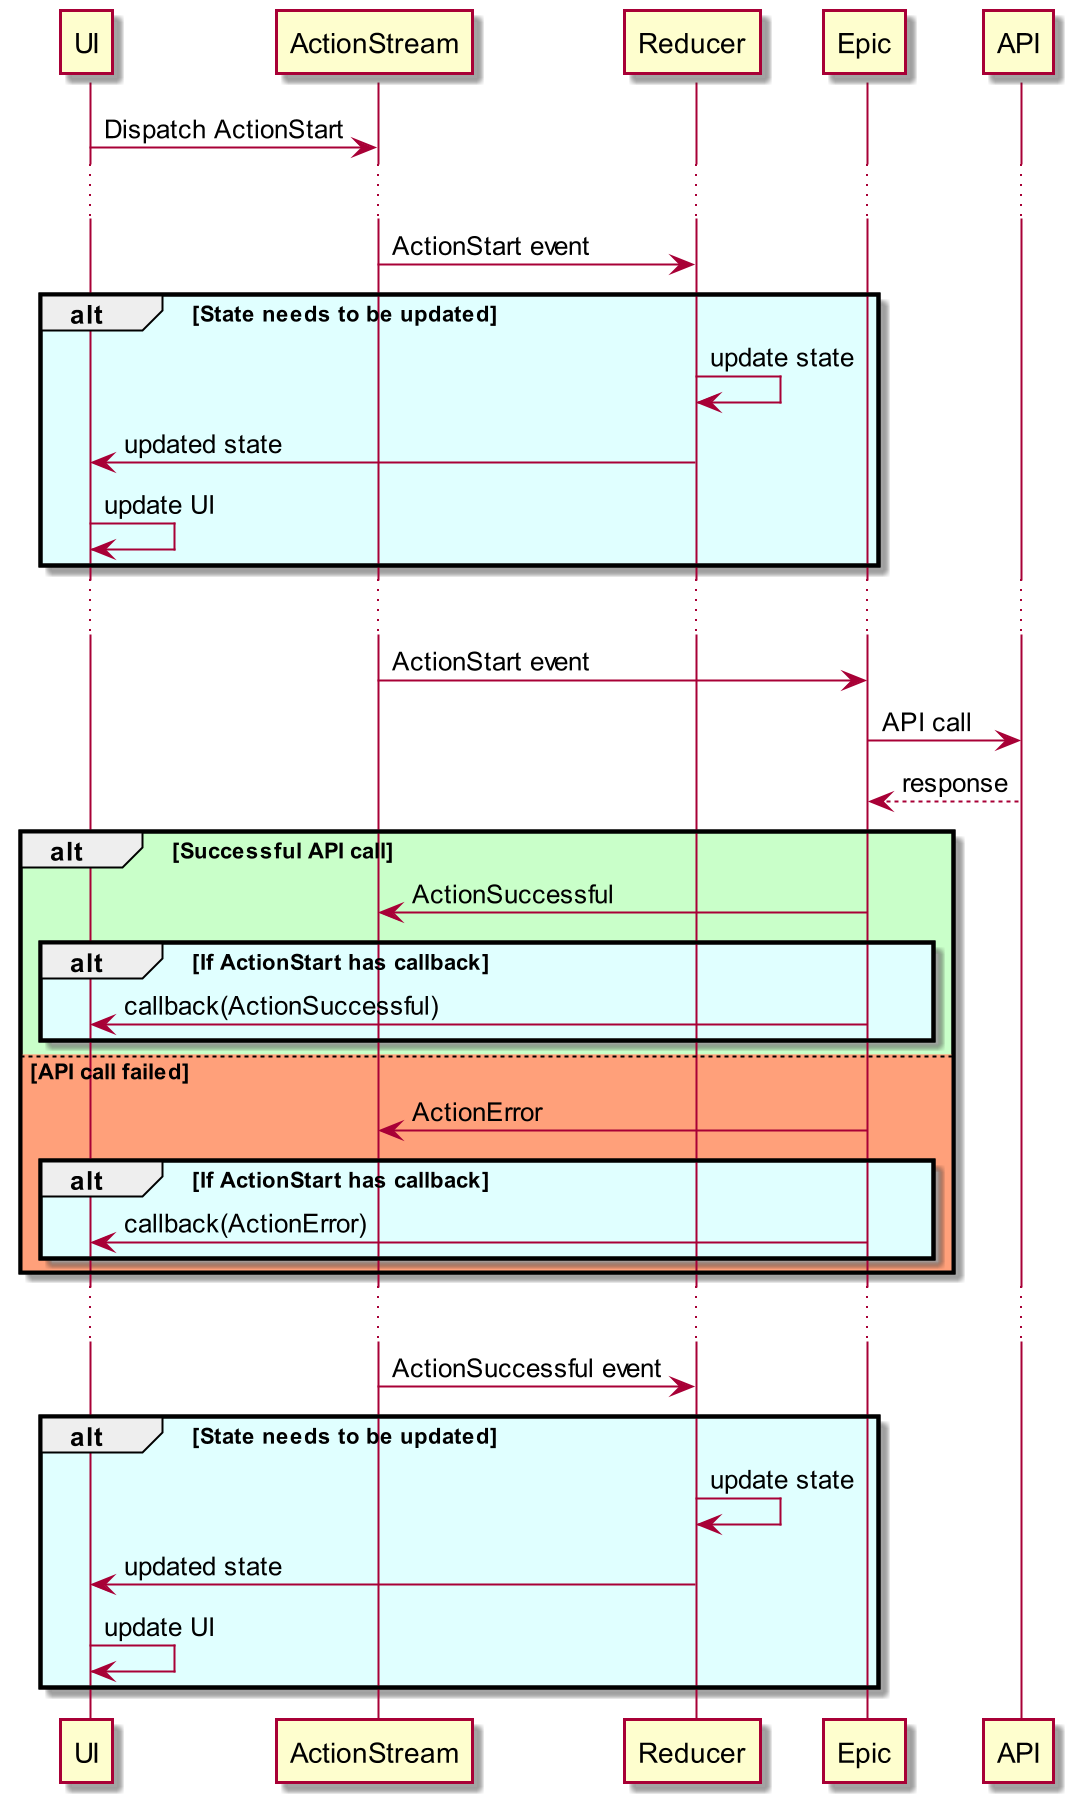
\includegraphics[scale=0.3]{diagrams/sequence/action.png}
    \caption{Sequence diagram of a generic normal action}\label{fig:action_sequence}
\end{figure}

In~\autoref{fig:action_sequence} I represented using a sequence diagram how a
generic normal action is processed by the application using in the redux
architecture. Some of the handlers have not been included into the diagram
because of size considerations but overall this is how most of the actions are
processed throughout the application.

An epic can also dispatch actions that are not part of the current process, for
example when creating a new password we want to also store it into the
permanent storage, thus the stream is expanded into the afferent
\textit{Success} action and a \textit{Start} action for the storage process.

\section{Application Models}

The data is represented by appropriate classes. All the passwords, codes and
OTP tokens toughener create a \textit{Bundle} of data.

\begin{figure}[H]
    \centering
    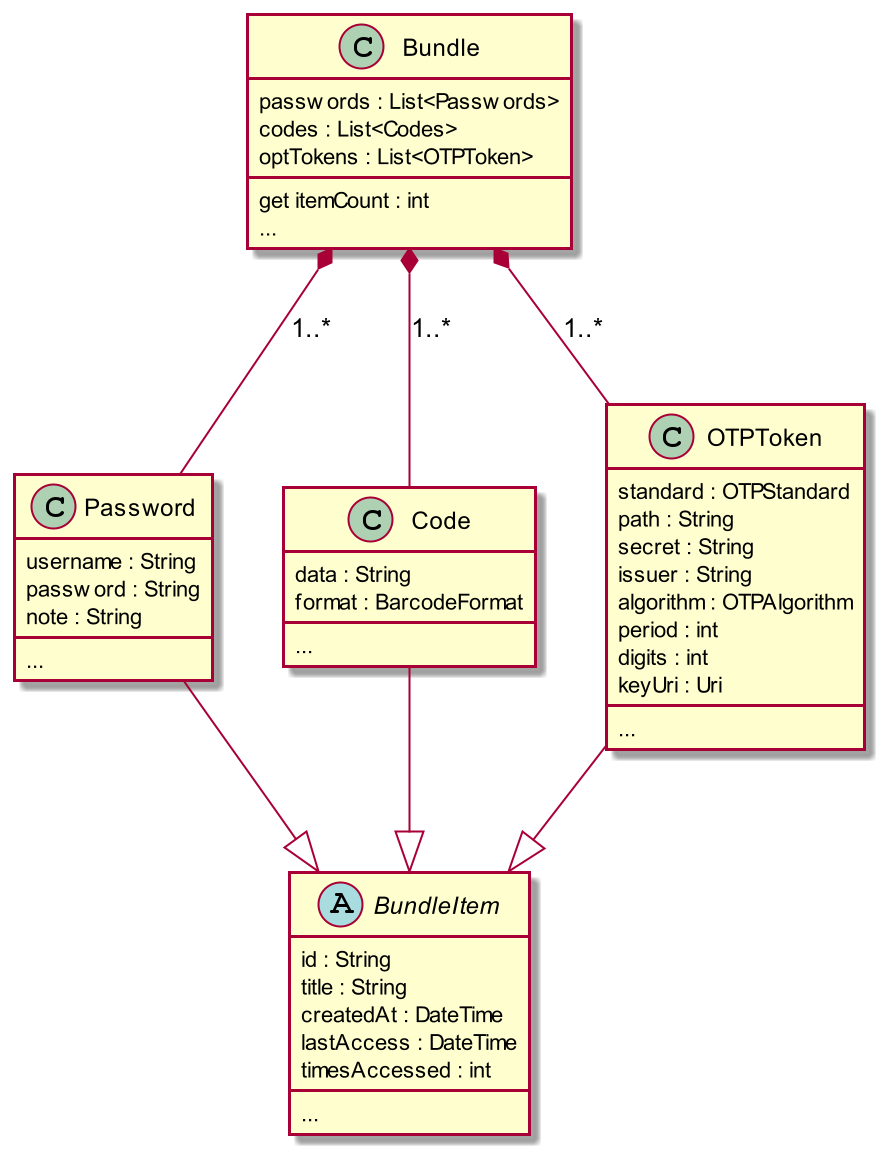
\includegraphics[scale=0.4]{diagrams/class/bundle.png}
    \caption{Class diagram of the Bundle model}\label{fig:bundle}
\end{figure}

A \textit{Bundle} contains a list of passwords, one of codes and a list of OTP
tokens as seen in~\autoref{fig:bundle}. The passwords, codes and tokens, all
implement the Bundle Item abstract class that contains general information
about them such as an unique id based on the UUID version 4
algorithm\cite{uuid} implemented into the uuid package\cite{uuidDocs}, title,
creation date and usage trends.

\begin{figure}[H]
    \centering
    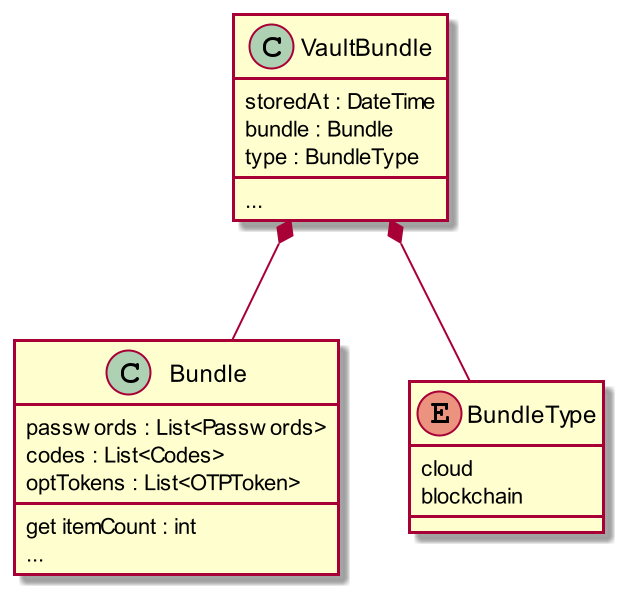
\includegraphics[scale=0.4]{diagrams/class/vault.png}
    \caption{Class diagram of Bundle element in backup storage}\label{fig:vault_bundle}
\end{figure}

A \textit{VaultBundle} is what is closer to what is stored on the blockchain.
As seen in~\autoref{fig:vault_bundle}, in addition to the bundle, storage date
and time and the type of storage are contained as well.

\section{Password Management}

Password management is one of the core functionalities of the application and
it is the most important feature. There are multiple operations that the user
can do related to password management and most of them are accessed from the
passwords fragment from the index page.

\subsection{Password Generator}

One of the features related to the password management is the password
generator.

\begin{figure}[H]
    \centering
    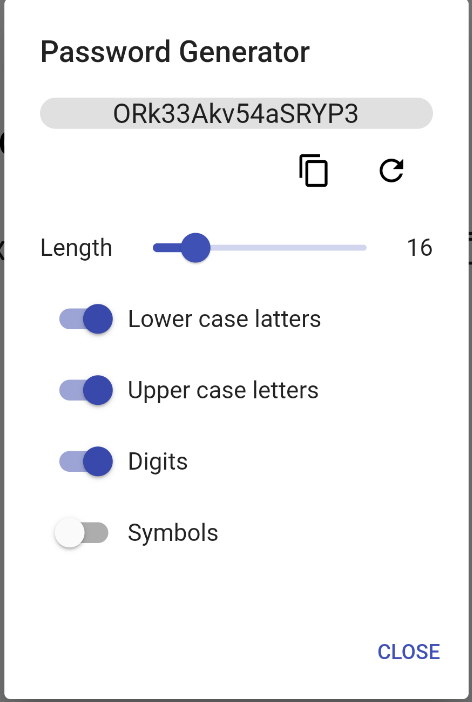
\includegraphics[scale=0.33]{images/app/password_generator.png}
    \caption{Password generator dialog}\label{fig:password_generator}
\end{figure}

In~\autoref{fig:password_generator} there is a screenshot with the password
generator dialog. As depicted into the image, the generator has two settings:
password length and character pool. When modified these settings are saved into
the state by appropriate actions. Every time the settings are changed, a
GeneratePassword action sequence is triggered in the epics. This action can
also be dispatched by the user by pressing the refresh button, and it is
automatically triggered when the generator dialog is opened. Instead of an API,
here the GeneratePasswordStart function calls an utility function with the
generator settings, which returns a random password based on the parameters.

\subsection{Create/Edit a Password}

\begin{figure}[H]
    \centering
    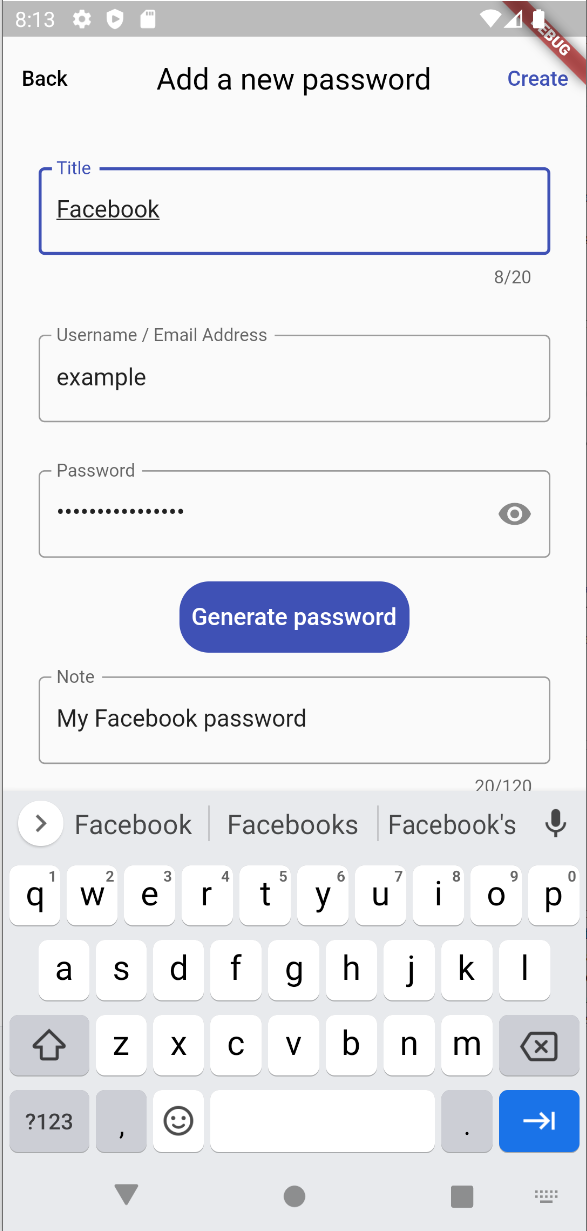
\includegraphics[scale=0.4]{images/app/new_password.png}
    \caption{New password page}\label{fig:new_password}
\end{figure}

When the user wants to create a new password they have to complete a form that
contains the password data. Here they have the option to use the password
generator in order to create a password which will automatically complete the
password field.

When the user taps on the create button a \textit{CreateNewPassword} action is
dispatched. This is a simple action that first updates the state in the reducer
and after that, in the epics, a new \textit{StoreBundleStart} action is
dispatched that will store the new password into the Secure Storage.

Editing a password is very similar with the creation process. The only
difference is that the first action replaces the existing password with the new
one instead of just adding it to the list.

\subsection{Delete a Password}

The user can delete the password from many different channels. The first one is
the long tap on the list element and the subsequent selection of the Delete
option form the context menu. Another one is pressing the delete button in the
edit page. There is also a button hidden into a slide action, similar with
deleting messages into an email application.

\begin{figure}[H]
    \centering
    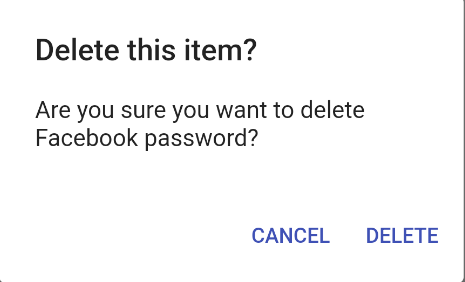
\includegraphics[scale=0.6]{images/app/warn_delete_password.png}
    \caption{Alert dialog with a warning that an item is about to be deleted}\label{fig:warn_delete_password}
\end{figure}

Whenever the user wants to delete a password they are shown a warning message
that the data will be lost that needs to be accepted. When the delete button is
pressed a DeletePassword action is dispatched and similar with the create and
edit ones it updates the state and triggers a bundle storage action.

\section{QR and Barcode Management}

\begin{figure}[H]
    \centering
    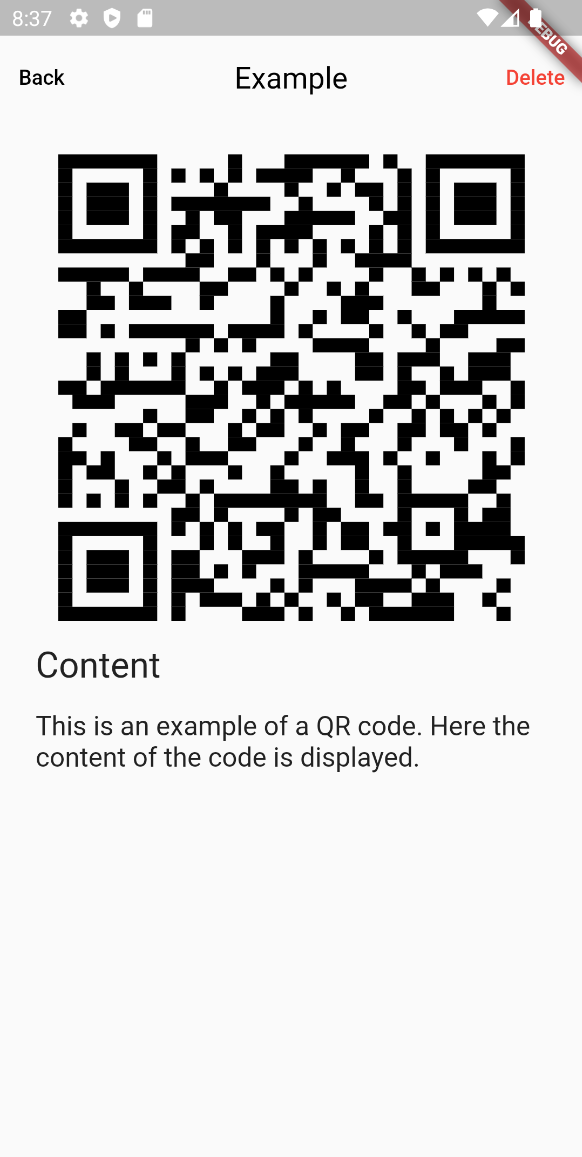
\includegraphics[scale=0.35]{images/app/view_qr.png}
    \caption{Code Details page}\label{fig:code_details}
\end{figure}

QR and Barcodes can be scanned, viewed and deleted.
In~\autoref{fig:code_details} we can see a QR code details page where the user
has a big image with the respective QR code generated and the content of the
code displayed.

When the user creates a new code a dedicated page is displayed where the user
is prompted to scan the code with the back camera of their mobile device. When
a code is detected, the page is swapped with another one in which the code is
displayed and the user needs to add a title. After the title is added a similar
process with the creation of a password happens and the code new is added to
the bundle.

Codes are scanned using the mobile\_scanner package~\cite{mobileScannerDocs}
which implements the scanning functionality of a QR or a barcode for dart. The
codes are then displayed using the barcode\_widget
package~\cite{barcodeWidgetDocs} which can generate a barcode of QR code of
different types from raw data. This way only the raw data and the algorithm
type are kept into permanent memory, reducing the storage size dramatically,
further reducing blockchain backup creation gas cost. No images are related to
QR or barcodes is stored.

\section{OTP Authenticator}

\begin{figure}[H]
    \centering
    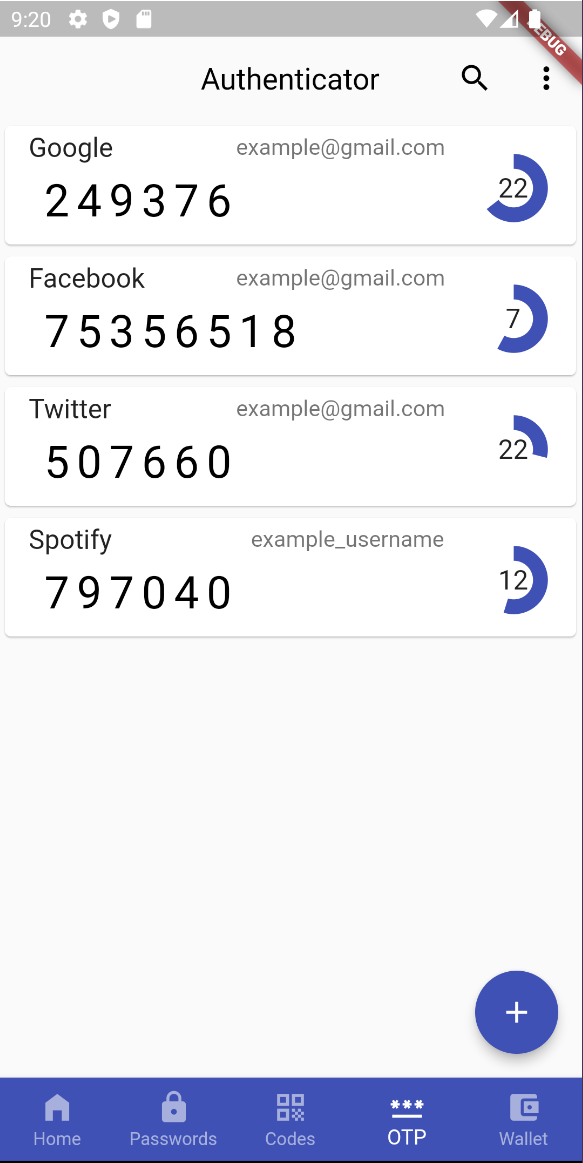
\includegraphics[scale=0.4]{images/app/tokens.png}
    \caption{OTP fragment from the index page}\label{fig:otp}
\end{figure}

The OTP authenticator functionality is the last piece of information that is
stored into the data bundle and is backed up. The creation process is similar
with creating a new Code but instead of entering a title, after scanning, the
title is automatically deduced based on the token. In~\autoref{fig:otp} is
shown the OTP fragment of the application where the list of tokens is
displayed.

The OTP tokens in~\autoref{fig:otp} have different parameters and their codes
are calculated correctly according to the TOTP specifications from~\cite{totp}.

HOTP tokens are not supported by the application. These tokens are usually used
on hardware implementations that don't have an exact clock and are considered
less secure. A HOTP could be converted into a TOTP, according to~\cite{totp}
the only difference is that the counter should be generated based on time, but
there is an issue with the server implementation of such a system which is not
guaranteed to increment the counter enough for it to find the current token.
The implementation of a true HOTP authenticator is basically included into the
implementation of the TOTP one according to~\cite{totp}, but I did not manage
to find a standardized QR code format for this type of token.

\subsection{TOTP}

\begin{figure}[H]
    \centering
    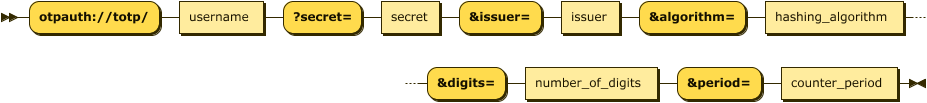
\includegraphics[scale=0.69]{diagrams/syntax/TOTP.png}
    \caption{Syntax diagram showing the anatomy of a TOTP token}\label{fig:totp_anatomy}
\end{figure}

A TOTP token contains the information needed to create an authentication code.
In~\autoref{fig:totp_anatomy} we can see the structure of a TOTP token. The
form of the token strongly resembles the URI format, some of the information
even being represented as query parameters.

The token starts withe the specification of what type of token it is. After
that the username for which the token was generated is provided. This username
can be an email address or just a string.

The query parameters don't have a specific order,~\autoref{fig:totp_anatomy}
shows just one of the possible arrangements. We start with the \textit{secret}
witch is the first query parameter in this case. The \textit{secret} is one of
the inputs into the HMAC function used to generate the key. The
\textit{algorithm} parameter specifies what hashing algorithm should be used to
generate the code. SHA1 is the most popular one from what I've seen, but MD5 or
SHA256 are also valid algorithms. The counter is created based on the
\textit{period} query parameter using the following simple formula:

\[counter=\frac{secondsSinceEpoch}{period}\]

The \textit{digits} query parameter specifies the length of the generated code.
And at last the \textit{issuer} is the entity who generated the token.

\begin{figure}[H]
    \centering
    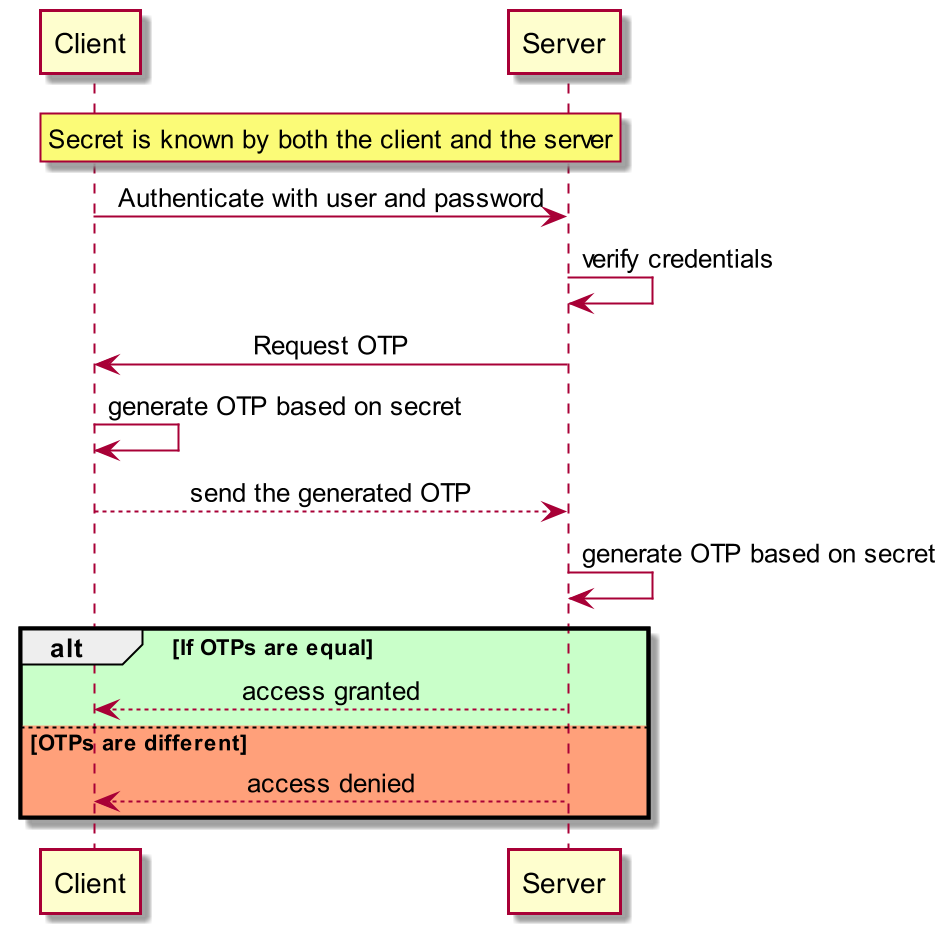
\includegraphics[scale=0.3]{diagrams/sequence/totp.png}
    \caption{Sequence diagram showing the basic concept of OTP authentication}\label{fig:totp_server_client}
\end{figure}

In~\autoref{fig:totp_server_client} I created a sequence diagram showing a
basic authentication scenario based on OTP two factor authentication. Both the
client and the server have previously shared the secret with each other (by
scanning a TOTP QR token) and they each generate a code which is validated by
the server.

\section{Cryptocurrency Wallet}

\section{Backup}

\subsection{Cloud Backup}

\subsection{Blockchain Backup}

\section{Security}

\chapter{Tests}

\section{Test Pipeline}

\section{Unit Tests}

\section{Widget Tests}

\section{Performance Statistics}

\chapter{Conclusions}

\section{Possible Improvements}

\bibliographystyle{plain}
\bibliography{references}
\addcontentsline{toc}{chapter}{Bibliography}

\end{document}